\chapter{System Architecture}

\section{UART Transceiver Architecture}

The UART Transceiver developed in this project is a modular digital design consisting of four major functional blocks: the UART Top module, Baud Rate Generator, UART Transmitter, and UART Receiver. The UART Top module integrates all submodules and controls the flow of data between the transmitter and receiver while sharing a common baud clock generated by the Baud Rate Generator.

The modular architecture improves design readability, simplifies verification, and allows individual modules to be synthesized and tested independently before integration. Such a hierarchical design methodology is commonly adopted in modern ASIC design to improve scalability and reusability.

\begin{figure}[!htbp]
    \centering
    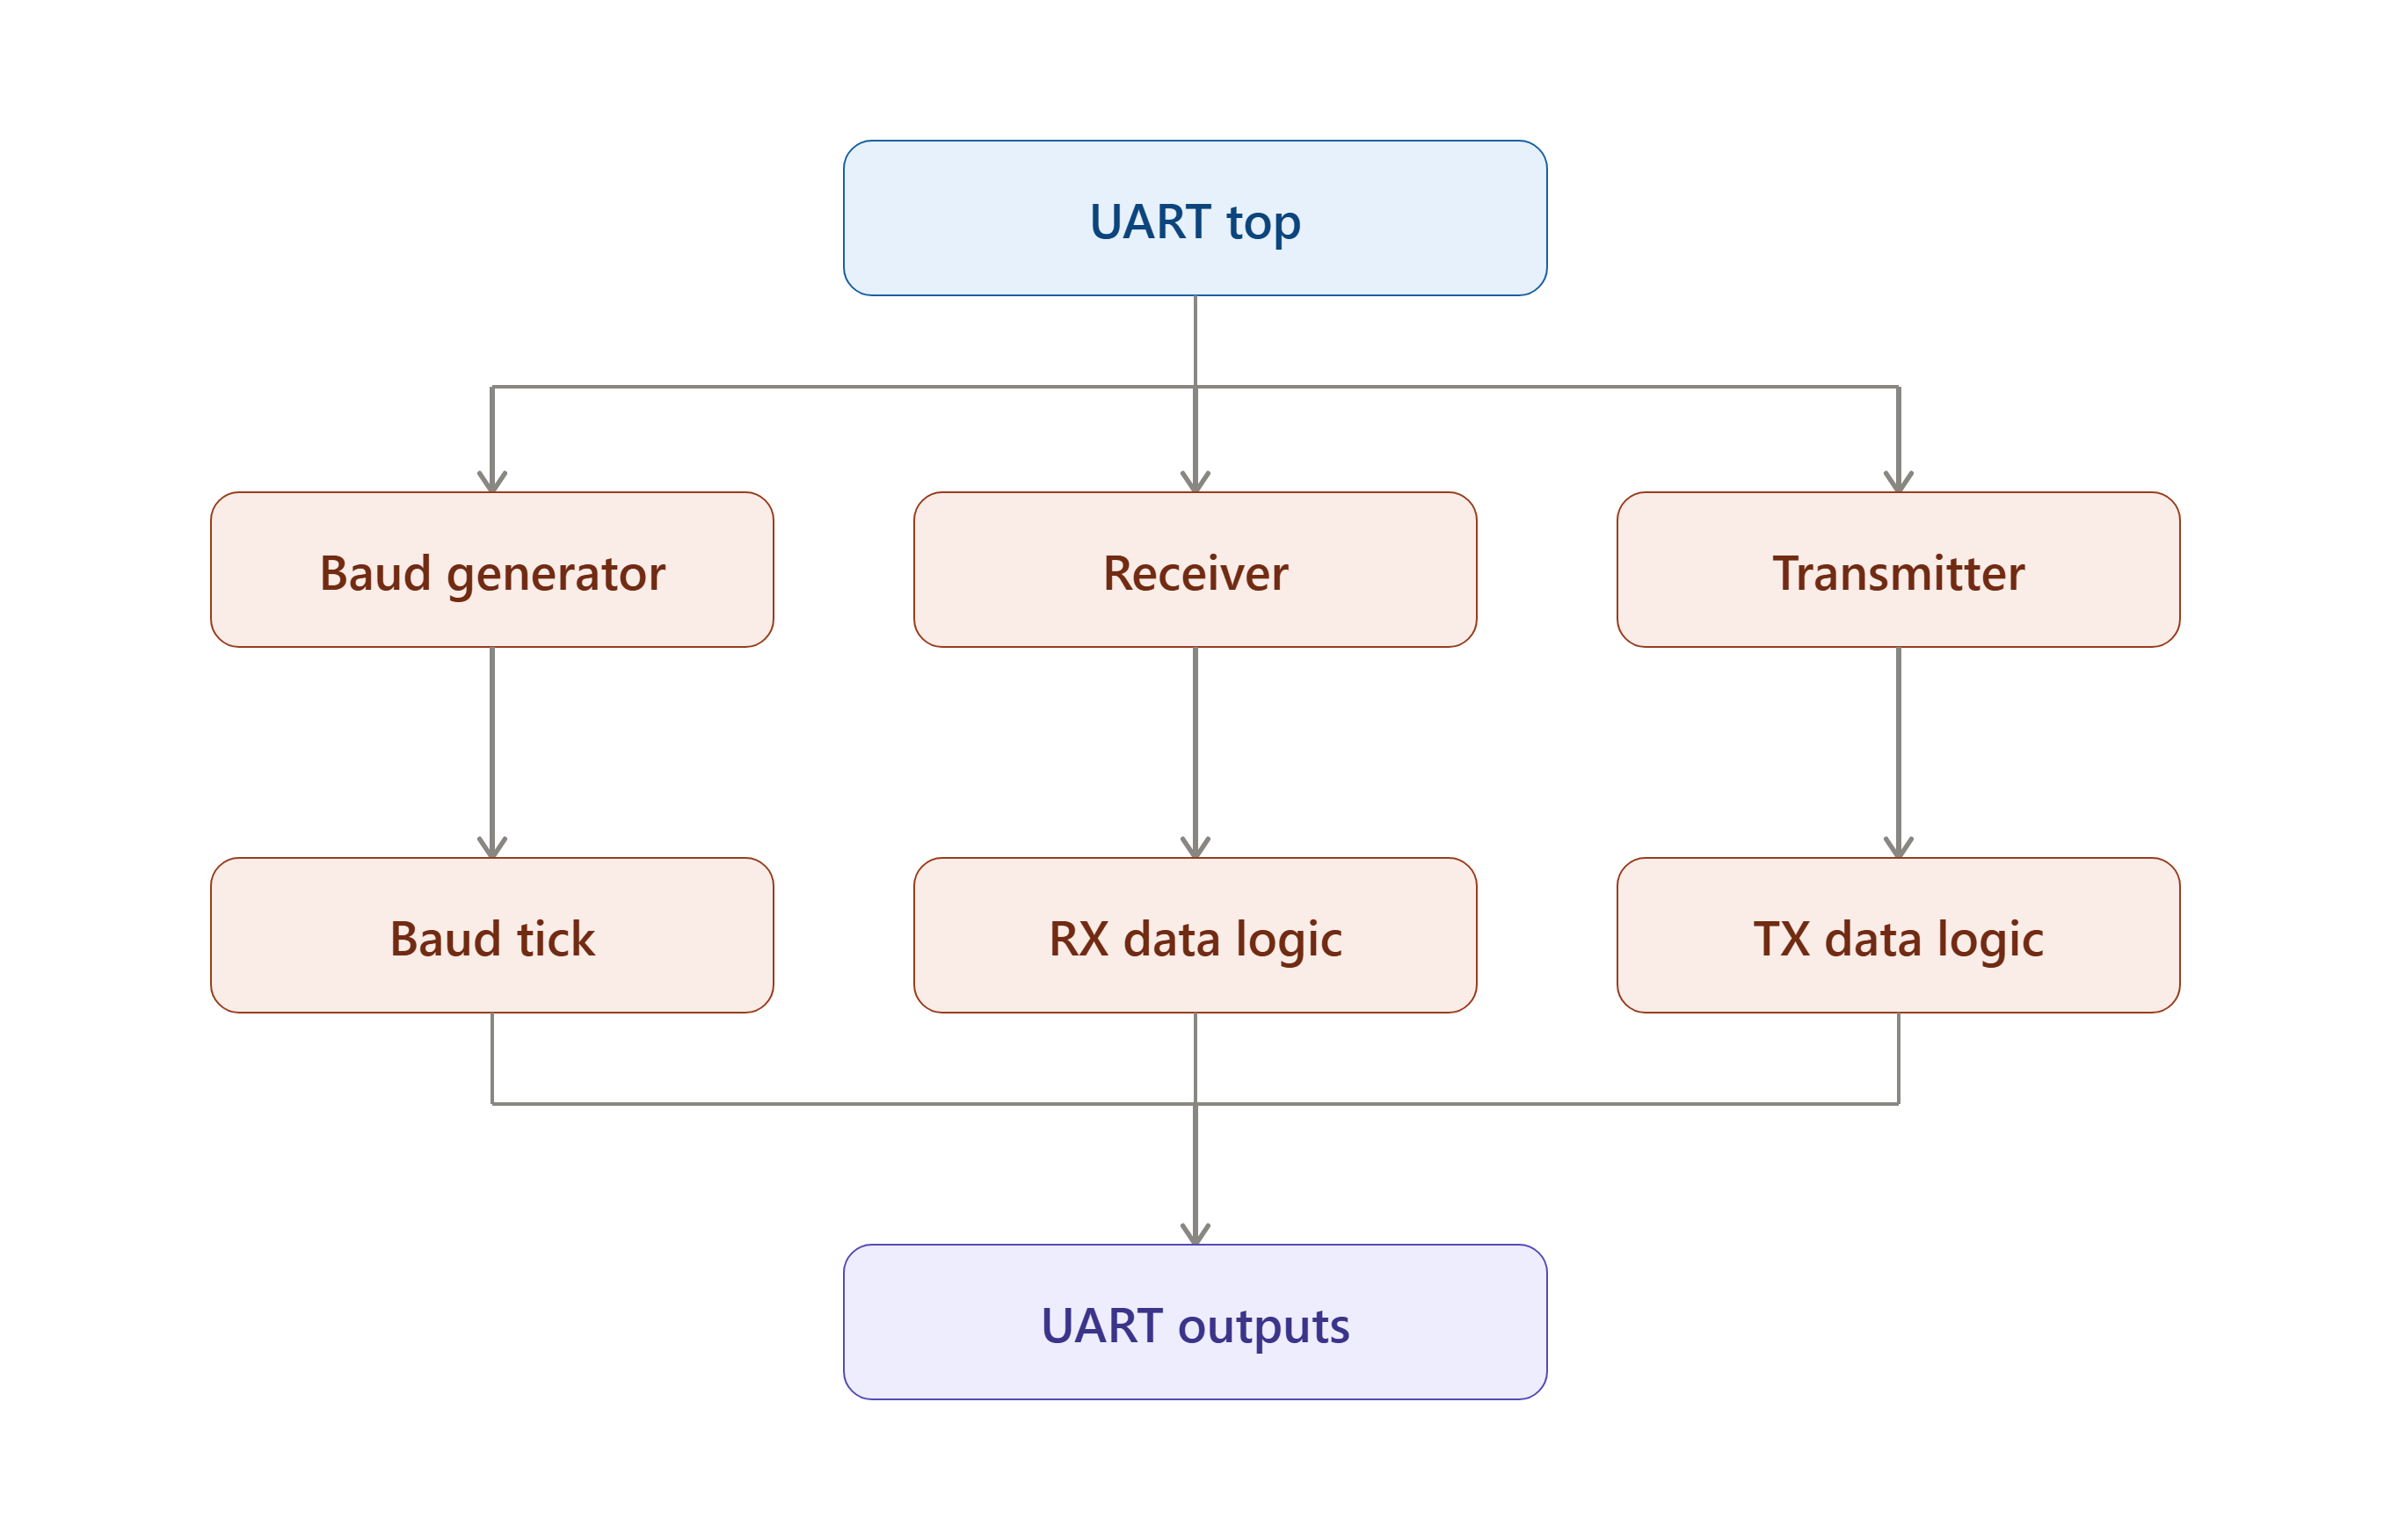
\includegraphics[width=0.88\linewidth]{images/uart_design_architecture.png}
    \caption{Top-Level Architecture of the UART Transceiver.}
    \label{fig:uart_top_architecture}
\end{figure}

Figure~\ref{fig:uart_top_architecture} illustrates the top-level organization of the UART Transceiver. The transmitter and receiver communicate through independent serial communication paths while both modules operate using the baud clock generated by the Baud Rate Generator.

%========================================================

\section{Internal Architecture}

Figure~\ref{fig:uart_internal_architecture} presents the complete internal architecture of the implemented UART Transceiver. The design consists of interconnected functional modules responsible for baud generation, serial transmission, serial reception, and top-level control.

\begin{figure}[!htbp]
    \centering
    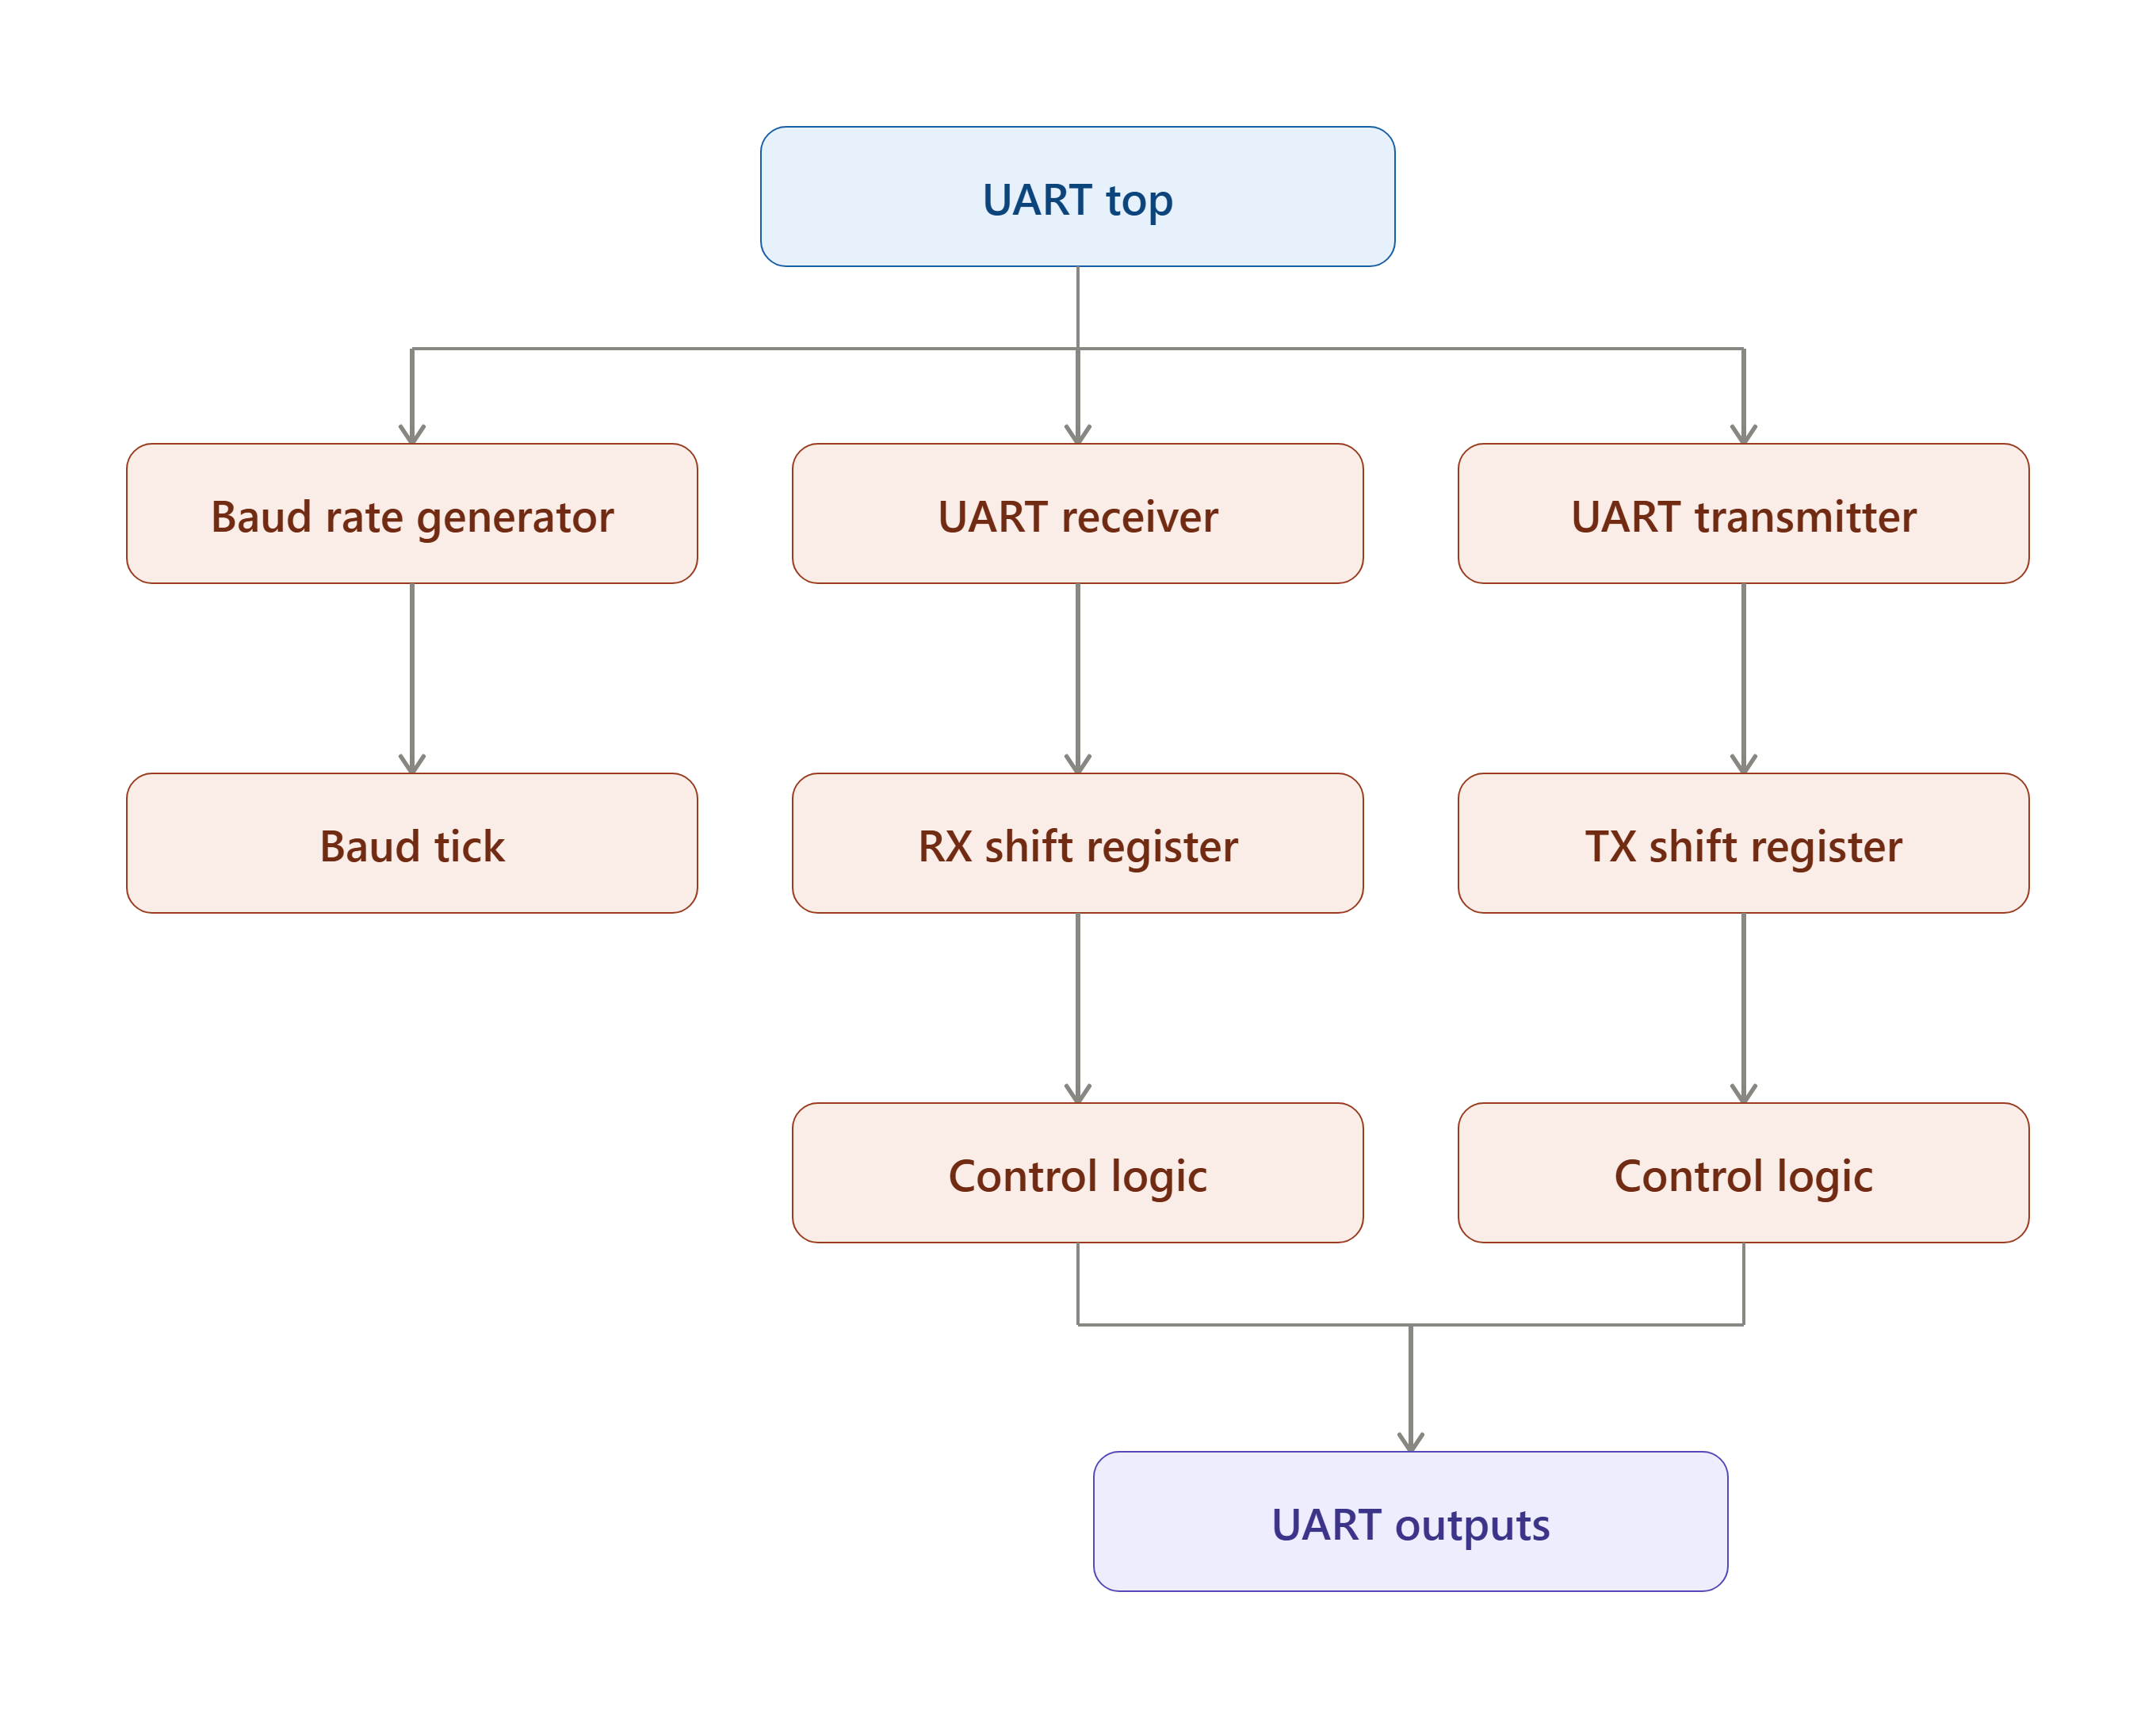
\includegraphics[width=0.92\linewidth]{images/complete_uart_internal_architecture.png}
    \caption{Internal Architecture of the UART Transceiver.}
    \label{fig:uart_internal_architecture}
\end{figure}

The hierarchical organization enables each module to perform a dedicated function while maintaining synchronized communication throughout the design. This approach simplifies debugging, verification, and future design modifications.

%========================================================

\section{Module Description}

Table~\ref{tab:uart_modules} summarizes the functionality of each major module implemented in the UART Transceiver.

\begin{table}[!htbp]
\centering
\caption{Functional Description of UART Modules}
\label{tab:uart_modules}

\renewcommand{\arraystretch}{1.3}

\begin{tabular}{|p{4cm}|p{9cm}|}

\hline

\textbf{Module} & \textbf{Function} \\

\hline

UART Top &
Integrates all functional modules and manages overall communication. \\

\hline

Baud Rate Generator &
Generates baud clock pulses from the system clock for synchronized data transmission and reception. \\

\hline

UART Transmitter &
Converts parallel input data into serial format according to the UART communication protocol. \\

\hline

UART Receiver &
Receives serial data and reconstructs the original parallel data while validating the received frame. \\

\hline

\end{tabular}

\end{table}

The following sections describe the architecture and operation of each module in detail.

%========================================================

\section{Baud Rate Generator}

The Baud Rate Generator is responsible for producing the baud clock required by both the UART transmitter and receiver. It divides the high-frequency system clock to generate timing pulses corresponding to the selected baud rate. Since both communication modules operate using the same baud timing, accurate baud generation is essential for reliable serial communication.

\begin{figure}[!htbp]
    \centering
    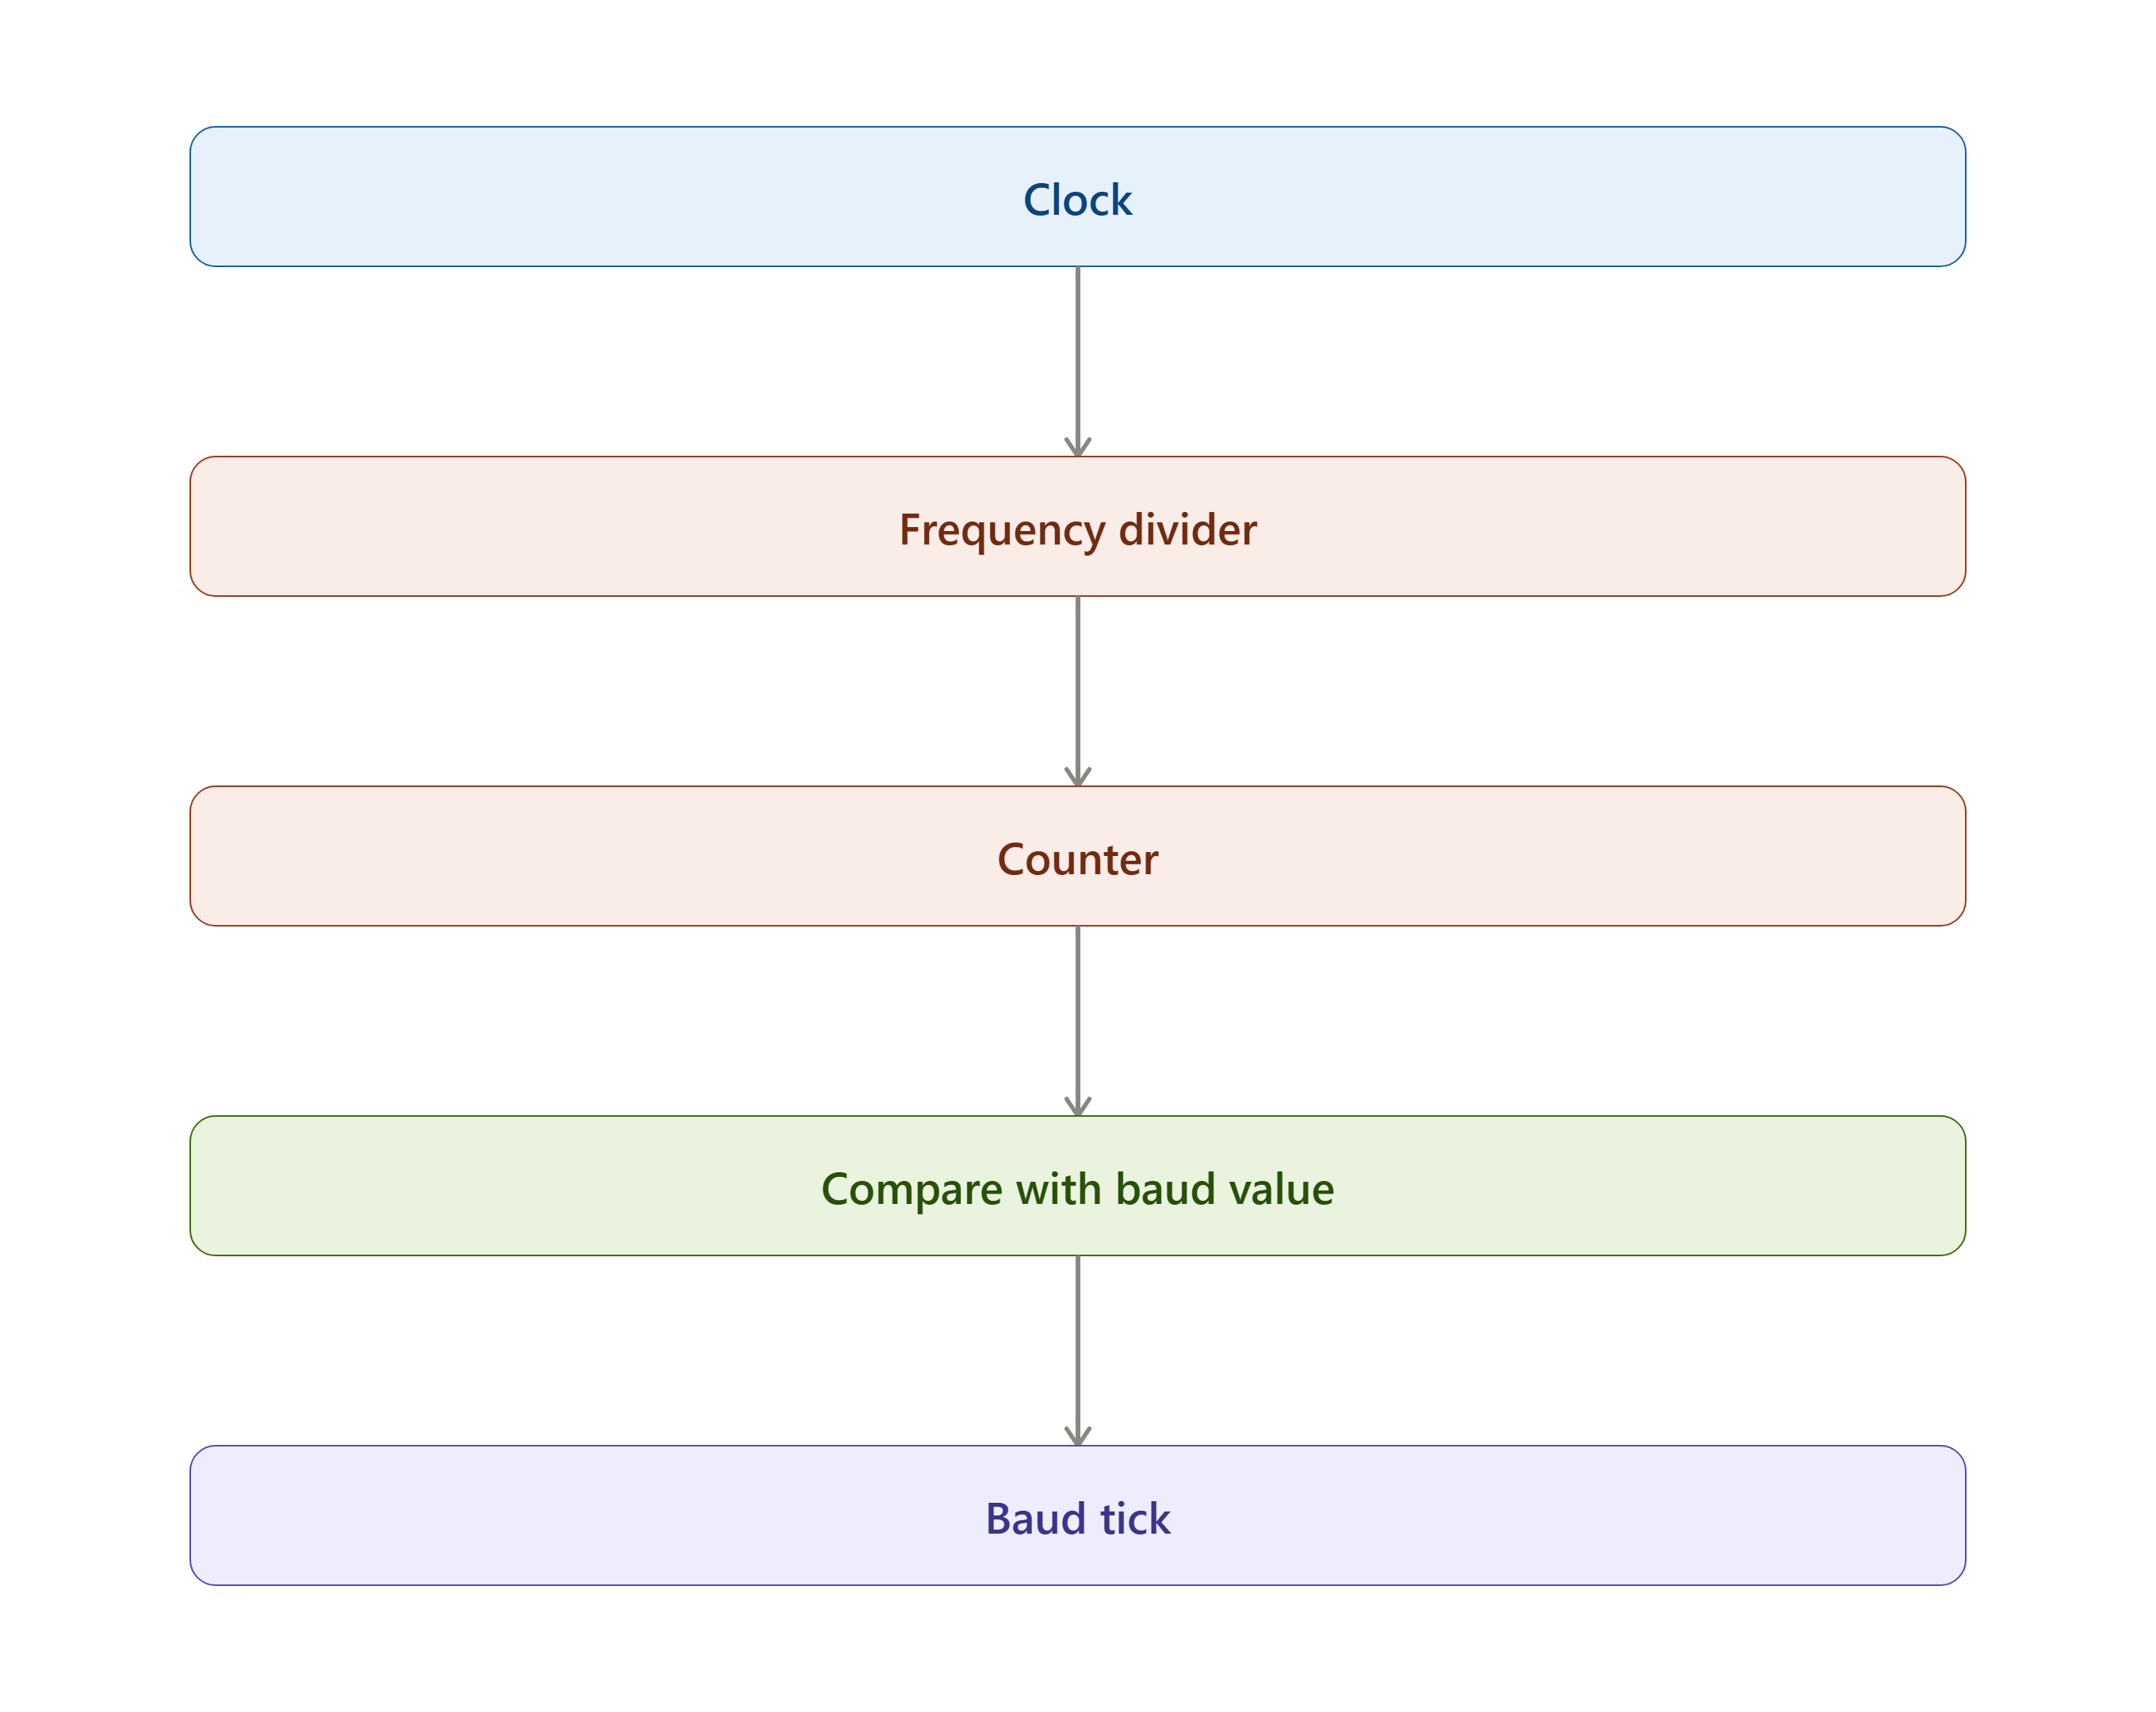
\includegraphics[width=0.80\linewidth]{images/baud_rate_generator_architecture.png}
    \caption{Architecture of the Baud Rate Generator.}
    \label{fig:baud_generator}
\end{figure}

The generated baud clock is distributed to both transmitter and receiver modules, ensuring synchronized operation throughout the communication process.

\clearpage

%========================================================

\section{UART Transmitter}

The UART Transmitter converts 8-bit parallel input data into a serial bit stream according to the UART communication protocol. Transmission begins only when the \texttt{tx\_start} control signal is asserted. The transmitter first sends the start bit, followed by the data bits in Least Significant Bit (LSB) first order, and finally transmits the stop bit to complete the communication frame.

The transmitter operates synchronously with the baud clock generated by the Baud Rate Generator, ensuring accurate timing for every transmitted bit.

\begin{figure}[!htbp]
    \centering
    \includegraphics[width=0.90\linewidth]{UART_Transmitter_Architecture}
    \caption{Architecture of the UART Transmitter.}
    \label{fig:uart_tx_architecture}
\end{figure}

Figure~\ref{fig:uart_tx_architecture} illustrates the internal organization of the transmitter module. The transmitter consists of control logic, shift registers, baud clock synchronization, and output logic that serializes the input data according to the UART protocol.

\vspace{0.3cm}

The major functions performed by the transmitter are:

\begin{itemize}

\item Accept 8-bit parallel input data.

\item Wait for the transmission enable signal.

\item Generate the start bit.

\item Shift data serially in LSB-first order.

\item Generate the stop bit.

\item Indicate transmission completion.

\end{itemize}

%========================================================

\subsection{Finite State Machine of UART Transmitter}

The transmitter operation is controlled by a Finite State Machine (FSM), which ensures that each communication frame follows the UART protocol correctly. The FSM sequentially controls the transmission of the start bit, data bits, and stop bit while maintaining synchronization with the baud clock.

\begin{figure}[!htbp]
\centering

\begin{tikzpicture}[
>=Stealth,
every node/.style={font=\small},
state/.style={circle,draw,thick,minimum size=1.3cm}
]

% States
\node[state] (idle) at (0,0) {IDLE};
\node[state] (start) at (3,0) {START};
\node[state] (data) at (7,0) {DATA};
\node[state] (stop) at (11,0) {STOP};

% Initial Arrow
\draw[->,thick] (-1.5,0) -- (idle);

% State Transitions
\draw[->,thick] (idle) -- node[above]{tx\_start} (start);

\draw[->,thick] (start) -- node[above]{baud\_tick} (data);

\draw[->,thick]
(data) edge[loop above]
node{More Data Bits} ();

\draw[->,thick] (data) -- node[above]{Last Bit} (stop);

\draw[->,thick,bend right=60]
(stop) to node[below]{baud\_tick} (idle);

\end{tikzpicture}

\caption{Finite State Machine of the UART Transmitter.}
\label{fig:tx_fsm}

\end{figure}

The transmitter FSM consists of the following operating states:

\begin{itemize}

\item \textbf{Idle} – Waits for the transmission request.

\item \textbf{Start} – Sends the start bit.

\item \textbf{Data} – Serially transmits the 8-bit data.

\item \textbf{Stop} – Sends the stop bit and returns to the Idle state.

\end{itemize}

The FSM guarantees that every transmitted frame follows the required UART timing and frame structure.

%========================================================

\section{UART Receiver}

The UART Receiver performs the reverse operation of the transmitter by converting incoming serial data into an 8-bit parallel output. The receiver continuously monitors the RX line and begins reception after detecting the falling edge of the start bit. Data bits are sampled according to the baud clock and reconstructed into the original parallel data.

Once all bits are successfully received, the receiver validates the stop bit before asserting the \texttt{rx\_done} signal to indicate successful reception.

\begin{figure}[!htbp]
\centering

\begin{tikzpicture}[
>=Stealth,
every node/.style={font=\small},
state/.style={circle,draw,thick,minimum size=1.3cm}
]

% States
\node[state] (idle) at (0,0) {IDLE};
\node[state] (start) at (3,0) {START};
\node[state] (data) at (7,0) {DATA};
\node[state] (stop) at (10,0) {STOP};

% Initial Arrow
\draw[->,thick] (-1.5,0) -- (idle);

% State Transitions
\draw[->,thick] (idle) -- node[above]{rx = 0} (start);

\draw[->,thick] (start) -- node[above]{Valid Start} (data);

% DATA loop
\draw[->,thick]
(data) edge[loop above]
node{Receive Next Bit} ();

% DATA -> STOP
\draw[->,thick]
(data) -- node[above]{Last Bit} (stop);

% STOP -> IDLE
\draw[->,thick,bend right=65]
(stop) to node[below]{Valid Stop} (idle);

\end{tikzpicture}

\caption{Finite State Machine of the UART Receiver.}
\label{fig:rx_fsm}

\end{figure}


\vspace{0.3cm}

The receiver performs the following functions:

\begin{itemize}

\item Detect the incoming start bit.

\item Sample serial data using the baud clock.

\item Reconstruct the original 8-bit parallel data.

\item Verify the stop bit.

\item Assert the reception completion signal.

\end{itemize}

%========================================================

\subsection{Finite State Machine of UART Receiver}

Similar to the transmitter, the receiver operation is governed by a Finite State Machine (FSM). The FSM synchronizes data sampling with the baud clock and controls the complete reception process from start-bit detection to successful frame completion.

The receiver FSM consists of four primary states:

\begin{itemize}

\item \textbf{Idle} – Waits for the detection of the start bit.

\item \textbf{Start} – Confirms the validity of the detected start bit.

\item \textbf{Data} – Samples and stores the incoming serial bits.

\item \textbf{Stop} – Verifies the stop bit and completes the reception process.

\end{itemize}

This state-based implementation ensures reliable data reception while minimizing synchronization errors during asynchronous communication.

\clearpage

%========================================================

\section{Data Transmission and Reception Flow}

The operation of the UART Transceiver can be divided into two independent processes: data transmission and data reception. Although both modules operate independently, they are synchronized using the baud clock generated by the Baud Rate Generator. The following flowcharts illustrate the sequence of operations performed during transmission and reception.

%--------------------------------------------------------

\subsection{UART Transmission Flow}

The transmission process begins when valid parallel data and the transmission enable signal are applied to the UART Transmitter. The transmitter serializes the data by generating the start bit, transmitting the eight data bits, and finally appending the stop bit before returning to the idle state.

\begin{figure}[!htbp]
\centering

\begin{tikzpicture}[
>=Stealth,
every node/.style={font=\small},
block/.style={
draw,
rectangle,
rounded corners,
minimum width=4.2cm,
minimum height=0.9cm,
align=center
}
]

% Blocks
\node[block] (start) at (0,0) {Start};

\node[block] (wait) at (0,-1.8)
{Wait for \texttt{tx\_start}};

\node[block] (startbit) at (0,-3.6)
{Transmit Start Bit (0)};

\node[block] (data) at (0,-5.4)
{Transmit Data Bits\\(LSB First)};

\node[block] (check) at (0,-7.2)
{All Data Bits Sent?};

\node[block] (stop) at (0,-9.0)
{Transmit Stop Bit (1)};

\node[block] (done) at (0,-10.8)
{Transmission Complete};

\node[block] (idle) at (0,-12.6)
{Return to IDLE};

% Arrows
\draw[->,thick] (start) -- (wait);

\draw[->,thick] (wait) -- node[right]{Yes} (startbit);

\draw[->,thick] (startbit) -- (data);

\draw[->,thick] (data) -- (check);

\draw[->,thick] (check) -- node[right]{Yes} (stop);

\draw[->,thick] (stop) -- (done);

\draw[->,thick] (done) -- (idle);

% No branch
\draw[->,thick]
(check.east) -- ++(2,0)
node[midway,below]{No}
-- ++(0,1.8)
-- (data.east);

\end{tikzpicture}

\caption{Flowchart of UART Data Transmission.}
\label{fig:tx_flowchart}

\end{figure}

Figure~\ref{fig:tx_flowchart} shows the sequential execution of the transmission process. Each state transition is synchronized with the baud clock to ensure accurate serial data transmission.

%--------------------------------------------------------

\subsection{UART Reception Flow}

The receiver continuously monitors the RX line for the detection of a valid start bit. Once detected, the receiver samples the incoming serial data using the baud clock, reconstructs the original 8-bit parallel data, verifies the stop bit, and asserts the reception complete signal.

\begin{figure}[!htbp]
\centering

\begin{tikzpicture}[
>=Stealth,
every node/.style={font=\small},
block/.style={
draw,
rectangle,
rounded corners,
minimum width=4.2cm,
minimum height=0.9cm,
align=center
}
]

% Blocks
\node[block] (start) at (0,0) {Start};

\node[block] (monitor) at (0,-1.8)
{Monitor RX Line};

\node[block] (detect) at (0,-3.6)
{Start Bit Detected?};

\node[block] (receive) at (0,-5.4)
{Receive Data Bits\\(LSB First)};

\node[block] (check) at (0,-7.2)
{All Data Bits Received?};

\node[block] (stop) at (0,-9.0)
{Check Stop Bit};

\node[block] (done) at (0,-10.8)
{Assert \texttt{rx\_done}};

\node[block] (idle) at (0,-12.6)
{Return to IDLE};

% Arrows
\draw[->,thick] (start) -- (monitor);

\draw[->,thick] (monitor) -- (detect);

\draw[->,thick] (detect) -- node[right]{Yes} (receive);

\draw[->,thick] (receive) -- (check);

\draw[->,thick] (check) -- node[right]{Yes} (stop);

\draw[->,thick] (stop) -- (done);

\draw[->,thick] (done) -- (idle);

% No branch from Detect
\draw[->,thick]
(detect.west) -- ++(-2,0)
node[midway,below]{No}
-- ++(0,1.8)
-- (monitor.west);

% No branch from Check
\draw[->,thick]
(check.east) -- ++(2,0)
node[midway,below]{No}
-- ++(0,1.8)
-- (receive.east);

\end{tikzpicture}

\caption{Flowchart of UART Data Reception.}
\label{fig:rx_flowchart}

\end{figure}

Figure~\ref{fig:rx_flowchart} illustrates the sequence followed by the receiver to recover the transmitted data while maintaining synchronization with the communication frame.

%========================================================

\section{Top Module Integration}

The UART Top module integrates the Baud Rate Generator, UART Transmitter, and UART Receiver into a single functional IP core. It distributes the baud clock to both communication modules, accepts parallel input data for transmission, receives serial input data, and provides the reconstructed parallel output.

\begin{figure}[!htbp]
\centering

\begin{tikzpicture}[
>=Stealth,
every node/.style={font=\small},
block/.style={
draw,
rectangle,
rounded corners,
minimum width=3.2cm,
minimum height=1.0cm,
align=center
}
]

%-------------------------------------------------
% Blocks
%-------------------------------------------------

\node[block] (baud) at (0,3)
{Baud Rate\\Generator};

\node[block] (tx) at (-5.5,0)
{UART\\Transmitter};

\node[block] (top) at (0,0)
{UART Top\\Module};

\node[block] (rx) at (5.5,0)
{UART\\Receiver};

%-------------------------------------------------
% Clock
%-------------------------------------------------

\draw[->,thick]
(-8,3) -- node[above]{clk} (baud.west);

%-------------------------------------------------
% Baud Tick
%-------------------------------------------------

\draw[->,thick]
(baud.south) -- node[right]{baud\_tick} (top.north);

%-------------------------------------------------
% Reset
%-------------------------------------------------

\draw[->,thick]
(-8,2) node[above]{rst} -| ([xshift=-4pt]tx.north);

%-------------------------------------------------
% TX Path
%-------------------------------------------------

\draw[->,thick]
(top.west) -- node[above]{tx\_data} (tx.east);

\draw[->,thick]
(tx.west) -- ++(-2,0)
node[midway,above]{TX};

%-------------------------------------------------
% RX Path
%-------------------------------------------------

\draw[->,thick]
(rx.east) -- ++(2,0)
node[midway,above]{RX};

\draw[->,thick]
(rx.west) -- node[above]{rx\_data} (top.east);

\end{tikzpicture}

\caption{Block Diagram of the UART Top Module.}
\label{fig:uart_top_block}

\end{figure}

Figure~\ref{fig:uart_top_flow} illustrates the interaction between all major functional modules within the UART Transceiver. The top-level controller coordinates the complete communication process by connecting the baud generation, transmission, and reception blocks.

%========================================================
The architecture presented in this chapter forms the basis of the RTL implementation described in the next chapter. The following chapter discusses the Verilog HDL implementation of each module along with functional simulation and verification prior to ASIC synthesis.

\clearpage